\documentclass[12pt, letterpaper]{article}
\usepackage[spanish]{babel}
\usepackage[utf8]{inputenc}
\usepackage{graphicx}
\usepackage{amssymb}
\graphicspath{{./imagenes/}}
\usepackage{xcolor}

%Paquetes para símbolos y entornos matematicos. En este documento se usa para poder usar el tag \begin{align} y \begin{align*} que permiten alinear expresiones matemáticas
\usepackage{amsmath}
\usepackage{amssymb}
%paquete que permite el uso de del argumento H al momento de insertar imágenes
\usepackage{float}

%comando para especificar el título del documento 
\title{Matemáticas para las Ciencias Aplicadas I}

%comando para especificar el autor del documento
\author{Pérez Romero Natalia Abigail}

%comando para especificar la fecha del documento
\date{\today}
%--------------Fin preámbulo--------------

%------------Inicio documento-------------
\begin{document}
%comando que genera el titulo con los datos especificados en el preámbulo
\maketitle
\textbf{Tarea X. Ejercicios del libro Cálculo. Una variable de Thomas J.R, George B.}

\textbf{Ejercicios 1, 5, 17, 43 y 79. de  la sección 2.4 Límites laterales y al infinito}

\textbf{1.} ¿Cuáles de las siguientes afirmaciones acerca de la función $y = f(x)$, cuya gráfica aparece a continuación, son verdaderas y cuáles falsas?\\


\begin{figure}[tbh]
\centering
\includegraphics[width=20em]{t11uno}
\end{figure}

\textbf{a.} $\lim_{ x \to -1^+} f(x) = 1$ .Es verdad\\
\textbf{b.} $\lim_{ x \to 0^+} f(x) = 0$ .Es verdad\\
\textbf{c.} $\lim_{ x \to 0^-} f(x) = 0$ .Es verdad\\
\textbf{d.} $\lim_{ x \to 0^-} f(x) =  \lim_{ x \to 0^+} f(x)$ .Es verdad\\
\textbf{e.} $\lim_{ x \to 0} f(x)$ existe. Es verdad\\
\textbf{f.} $\lim_{ x \to 0} f(x) = 0$ Es verdad\\
\textbf{g.} $\lim_{ x \to 0} f(x) = 1$ Es falso\\
\textbf{h.} $\lim_{ x \to 1} f(x) = 1$ Es falso\\
\textbf{i.} $\lim_{ x \to 1} f(x) = 0$ Es falso\\
\textbf{j.} $\lim_{ x \to 2^-} f(x) = 2$ Es verdad\\
\textbf{k.} $\lim_{ x \to -1^-} f(x) $ no existe. Es verdad\\
\textbf{l.} $\lim_{ x \to 2^+} f(x) = 0$ Es falso\\



\begin{figure}[tbh]
\centering
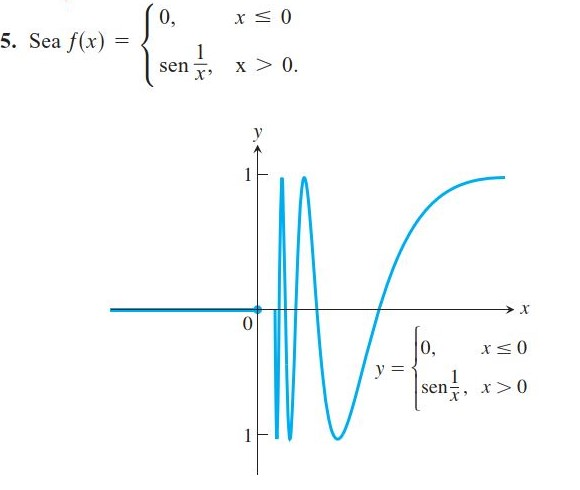
\includegraphics[width=20em]{t11dos}
\end{figure}


\textbf{a.} ¿  $\lim_{ x \to 0^+} f(x)$ existe? No, porqué la función $\sen \frac{1}{x}$ tiene muchas intersecciones con el eje x. Cuando $x \to 0$, los valores de $ \sen (1/x)$ se repiten peródicamente entre -1 y 1. No hay un solo número L al que los valores de la función estén suficientemente cercanos cuando $x$ se aproxima a cero.


\textbf{b.} ¿ $\lim_{ x \to 0^-} f(x)$ existe? Sí $\lim_{ x \to 0^-} f(x) = 0$, porque cuando se aproxima el límite por la izquierda la función es una constante.


\textbf{c.} ¿ $\lim_{ x \to 0} f(x)$ existe? No, a pesar de que $\lim_{ x \to 0^-} f(x)$ existe, el $\lim_{ x \to 0^+} f(x)$ no existe, por definición para decir que rl límite existe los límites laterales deben ser iguales.

\textbf{17.} Encuentre los límites

$\lim_{x \to -2^+} (x+3) \frac{|x+2|}{x+2} = \lim_{x \to -2^+} \frac{(x+3)}{1}\frac{|x+2|}{x+2} = \frac{(x+3)(|x+2|)}{x+2}$ 


\begin{figure}[tbh]
\centering
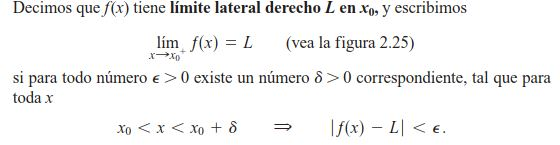
\includegraphics[width=20em]{t11tres}
\end{figure}



\end{document} 